\documentclass[authoryear]{elsarticle}
\usepackage{tabulary}
\usepackage{eurosym}

\makeatletter
\g@addto@macro\@floatboxreset\centering
\makeatother

\begin{document}

\title{A History of Downtown Congestion Pricing}
\author[ll]{Lewis Lehe \corref{cor1}}

\address[ll]{UC Berkeley, Department of Civil and Environmental Engineering \\ lewis500@berkeley.edu \\ http://lewislehe.com}

\begin{abstract}

Downtown congestion pricing (DCP) is the practice of charging tolls on driving in a city's central areas as a way to relieve traffic congestion. Five major cities have implemented DCP: Singapore, London, Stockholm, Milan and Gothenburg. This paper reviews the history of DCP from the 1950's to the present-day. It describes each scheme's implementation, design, transportation impacts and finances as well as some outside historical developments. Along the way, two themes are noted: First, that exemptions from charging are highly consequential, as exempt traffic quickly grows after tolls are put in place. Second, that instituting a toll discourages much more traffic than increasing one does.

\end{abstract}

\maketitle

\section{Introduction}

Today, authorities in Vancouver and New York City are considering implementing tolls on zones of their downtown street networks as a means of relieving traffic congestion---a practice we will call ``downtown congestion pricing'' (DCP). Forms of congestion pricing are already in place on highways and bridges throughout North America, such as Highway 407 in Toronto and the High-Occupancy Toll (or ``Express'') Lanes now proliferating across the United States. But the schemes being considered for New York City and Vancouver would differ from not only by their setting but also topologically: while congestion pricing on highways charges drivers to travel between well-defined start and end points, DCP charges for use of  clusters of contiguous downtown streets (``zones''); charged trips can thus begin and end at numerous points within the zone or along its boundary. Thus, DCP is attended by administrative and technological concerns that warrant special treatment.

To date, only five cities have implented DCP as we have defined it: Singapore, London, Stockholm, Gothenburg and Milan. This paper provides a broad sweep of their experiences along with some historical connective tissue. The goal is to help the reader quickly become familiar with the experience of DCP thus far and to point toward works containing further information. Similarly, \citet{Hau1992}, \citet{Gomez-Ibanez1994}, \citet{Small1998} and \citet{Anas2011} survey various congestion pricing schemes up to their publications, with \citet{Gomez-Ibanez1994} being especially thorough, but this paper includes later developments and emphasizes the special concerns of downtown schemes.

\subsection{Organization and scope}

We describe six DCP schemes: Singapore's Area License Scheme (\ref{sec:als}), Singapore's Electronic Road Pricing (Sec. \ref{sec:erp}), the London Congestion Charge (Sec. \ref{sec:london}), the Stockholm Congestion Tax (Sec. \ref{sec:stockholm}), Milan's Ecopass and Area C\footnote{These are treated together as Area C is technologically the same as Ecopass but has different prices and exemptions.} (Sec. \ref{sec:milan}) and the Gothenburg Congestion Tax (Sec. \ref{sec:gothenburg}). Each description includes four subsections:

\begin{enumerate}
    \item \emph{Implementation}. Motivation and events leading up to implementation.
    \item \emph{Design}. The scheme's technology, prices, exemptions and geography---including changes over time.\footnote{In these sections, details about scheme design comes from the schemes' official websites except when otherwise noted.}
    \item \emph{Transportation Impacts}. Impact on travel---especially on the magnitude and composition of flow into the charged zone and, where available, on speeds and transit ridership. Note that DCP also affects air pollution, equity, real estate and commerce. But the transportation impacts are the most well documented, comparable and, arguably, \emph{direct} impacts. The reader interested in other effects---which are undoubtedly important---can usually find such information in the works cited.
    \item \emph{Finances}. How much money the scheme has cost to build and operate, and how much revenue it has raised.
\end{enumerate}

In between are sections devoted to historical context. Sec. \ref{sec:early} describes intelletual developments prior to real implementation. Sec. \ref{sec:transition} describes a twenty-year ``transition period'' following Singapore's first scheme. Sec. \ref{sec:future} briefly describes future plans. 

Note that, for brevity and focus, certain developments in the history of DCP have been omitted. For example, Valetta, Malta \citep{Attard2010} and Durham, England \citep[p.269]{Santos2006a} also apply tolls to central areas, but these schemes are very small and not much data is collected on their outcomes. 

% Likewise, about ten schemes were proposed but languished or been cancelled (including Hong Kong, Edinburgh, Manchester, New York City, San Francisco, Cambridge, the Randstadt region of the Netherlands and Helsinki), but among these only Hong Kong's is discussed, because it provides context for Singapore's ERP.

\subsection{Themes}\label{ssec:themes}

The paper is more focused on description than inference, but we do point out two recurring themes.

Theme I is that exemptions are among the most consequential aspects of a scheme's design, to a degree that often surprises authorities. Exempt classes of trips or vehicles quickly become a large share of traffic, and in doing so they compromise congestion goals and reduce revenue more than projected.

Theme II is that charging implementing a toll is much more consequential than differences in the toll level. When a scheme is implemented, entries to the tolled zone by vehicles subject to charge drop sharply, but later toll increases make only a minor difference. Noting this effect in Stockholm and Gothenburg, \citet[p. 45]{Borjesson2018} offer two explanations. The first is grounded in traditional economic theory: the initial toll discourages all the drivers with elastic demands, so the traffic exposed to later toll increases is composed of drivers with a high willingness-to-pay for travel. The second explanation is grounded in behavioral economics: \citet{Shampanier2007} note that consumers are extremely sensitive to being charged \emph{any} positive price---even negligible ones.


\section{Early steps}

This section treats a period from the mid 1950's until the early 1970's, during which the idea of pricing urban areas was incubated. The section concludes by pointing out a family resemblance between how British scholars of that era conceived of traffic in towns and how they planned workable pricing schemes.

\citet{buchanan1952} makes passing mention of a ``city license,'' while \citet{Walters1954} explains in more detail: ``For example, a special `London licence' would have to be acquired and displayed before vehicles could use the roads of central London between 8 a.m. and 6 p.m.'' But the first detailed proposal for downtown pricing came in a 1959 testimony to the US Congress by the economist William Vickrey \citep{Vickrey1959}. Vickrey's testimony is, in part, a response to a difficulty posed by Dick Netzer of the Federal Reserve Bank of Chicago four years ealier:
\begin{quote}
 We cannot construct a tollgate at each and every intersection, and there is no way of metering highway service---like electric or water service, for example---that would take a meter on each vehicle which records only only the mileage but the kind of road used, the time of day, and so on. (\citet{Netzer1955} quoted in \citet{Vickrey1959})
\end{quote}

Vickrey's answer was wireless, electronic tolling that would obviate the need for congestion-inducing tollbooths. The Washington, D.C. metropolitan area would be divided into a large number of zones (``between 60 and 200''), and cars would carry transponders. Along the borders of the pricing zones, interrogators would signal the transponders on passing cars with electromagnetic waves, whereupon the transponders would return an identifying signal---essentially the concept behind RFID-based electronic tolling that is widespread today. Selective camera enforcement would do for cars without transponders. Remarkably, Vickrey not only supplied detailed costs and technical specifications for much of the system---from transmission to data storage---but actually demonstrated the transponder apparatus for Congress using a model train set-up.\footnote{Richard Arnott and Marvin Krauss later cleaned up Vickrey's testimony and published it as \citet{Vickrey1994}, but the author has obtained the original document and can supply it on request.} 

At the same time Vickrey was at work on Washington's problems, British officials perceived their own country to be approaching a traffic crisis: the number of registered vehicles had doubled from 4.5 million in 1950 to 9 million in 1960, but state expenditure on roads was low, and there was as yet no motorway network \citep[p.523-524]{Gunn2011}. While building motorways could be hoped to alleviate intercity congestion, urban traffic in Britain's old cities remained an unsolved and growing problem. Therefore, in 1960, the UK government commissioned the urban planner Colin Buchanan, who had written a book on cars in cities, to analyze the question of city traffic and propose planning remedies. 

Other British researchers, however, thought that road pricing held more promise than reconfiguring city streets and land-use---particularly for cities where the cost of construction was high and the extant road network ancient.\footnote{See \citep{Rooney2014} for an account of the ideological conflict between the planning and pricing approaches to managing urban traffic during this era.} Gabriel Roth, a researcher at Cambridge, asked, ``Before pulling down the fabric of the country let us at least consider the economic implications of what we are doing'' \citep[p.289]{Roth1961}. The same year, Walters published \citet{Walters1961}---one of the most cited works in transportation economics---which couched orthodox relations among flow and speed in terms of the supply-and-demand diagram of microeconomics. While focused on highways, the paper mentions pricing might be applied to city streets using a special mileometer, which---once the driver turned it on---would display a flag that roadside observers could check.

In July 1962, the Ministry of Transport convened a group of researchers to discuss road pricing, whereafter officials established a committee---helmed by Reuben Smeed of the UK's Road Research Laboratory and including Alan Walters and Gabriel Roth---to write a report on road pricing \citep{Rooney2014}. After a series of meetings, the report---commonly referred to as the ``Smeed Report''---was published in July 1964. The Smeed Report, \citet{MoT1964}, sets out principles for a good urban road pricing system and proposes a large number of schemes with varying levels of technical complexity. These schemes include simple parking surcharges, daily licenses (pieces of paper or stickers that must be displayed to enter certain zone), electronic systems like Vickrey's, and systems where drivers activate timers or mileometers when they travel through congested areas. For instance, one system DESCRIBE THE COLORED LIGHT SYSTEM.


Ultimately, the report was unpopular with the government. INCLUDE DETAILS LATER. OVERSHADOWED BY BUCHANAN.

Still, scholarly work on pricing continued apace (CITE SOME EXAMPLES). The World Bank commissioned a study by the US Consultancy Alan M. Vorhees for road pricing in Caracas, Venezuela \citep{Vorhees1973}, which would seem to have influenced Singapore's decision to adopt road pricing, discussed below.

% \subsection*{The idea of zones}

% TALK HERE ABOUT ALL THE ZONE SCHEMES. THEY DIDN"T SEEM TO ACIVELY ACKNOWLEDGE THE CRUCIAL DIFFERENCE BETWEEN A ZONE AND A LINK, BUT AT THE SAME TIME THEY WERE DOING RESEARCH ON ZONAL RELATIONS.
A characteristic common to many of the schemes is the division of cities into zones, where the zones with the highest demand for road travel would be the most expensive to traverse. 

One heretofore neglected aspect of this line of thought is that, at the same time British researchers were coming up with schemes to price cities by the zone, they were also developing a macroscopic 

\section{Singapore Area License Scheme}

% \subsection{History}

The motive for Singapore's interest in road pricing was similar to that of Britain's: explosive growth in car ownership. Between 1960 and 1970, the private vehicle population of Singapore doubled as the country grew wealthier and began to develop large residential estates in the island's hinterlands, but the total length of public roads rose only 35\% \citep[p.211-212]{Santos2004}. In response, throughout the 1970's the government undertook a menu of forceful policies which included: consolidating myriad bus operators into a single national company, a six-fold increase in road spending from 1975 to 1980, and high, escalating taxes on car purchases\footnote{See Appendix B of \citet{Gomez-Ibanez1994} for a list of  policies against car ownership.} \citep{Santos2004}. 

In 1973, the Singapore government convened the Road Transport Action Committee (RTAC) to propose solutions to congestion. The Committee's first proposals included bus lanes as well as efforts to encourage staggered work hours (especially for public employees) and carpooling \citep{Chin1998}. In May 1974 the RTAC published a report, \emph{A Plan for the Relief of Traffic Congestion in the City}, declaring, ``Singapore cannot afford to continue to allocate scarce and valuable land to build unlimited miles of roads to keep pace with this uncontrolled increase in traffic'' \citep[p.3]{SRTAC1974}. The plan proposed four policies: (i) sharp increases in CBD parking rates; (ii) new commuter bus services; (iii) a park-and-ride scheme whereby commuters would park in garages outside the CBD and take special shuttles to their workplaces; (iv) the Area License Scheme---a simple supplementary license system that made up the core of the plan.\footnote{It is possible the idea for ALS came when Gabriel Roth (of the Smeed committee), who was then working in Singapore as a consultant for the World Bank, passed the World Bank's plan for road pricing in Caracas, \citet{Vorhees1973}, to members of the RTAC (CITE ROTH 1996).} The Area License Scheme commenced operation on June 3, 1975 and continued until 1997, when an electronic system replaced it.

\subsection{Design}

At post offices, gas stations, convenience stores and roadside booths located along roads leading into the RZ, drivers paid S\$3 to buy a daily ``license'', or S\$60 for a monthly one, that permitted them to enter to a 6.2 km$^{2}$ Restricted Zone (RZ), Monday through Saturday morning \citep{WatsonHolland1978}. The ``license'' was a paper decal that went in the windshield. Wardens at 22 access points wrote down the plate numbers of vehicles lacking licenses. At first, only private vehicles with fewer than three passengers had to show licenses; taxis, commercial goods vehicles, public vehicles, motorcycles, carpools and buses were exempt, but taxis lost their exemption within three weeks. While the charging period was 7:30-9:30 AM originally, authorities noticed a surge of traffic just after 9:30 AM and extended charging to 10:15 AM starting August 1, 1975. The Park-and-Ride scheme was essentially shut down within a few months for lack of ridership, and the new bus services did not draw many customers. 

There were many changes to ALS over the years.\footnote{See Table 1 of \citet[p. 98]{PhangToh1997} for a table listing the nature and dates of modifications to ALS. } In 1976, the price of a license was increased to S\$4 and a double rate charged to registered company cars, because firms were able to deduct the ALS as a business expense. In 1977, charges for taxis were cut to S\$2, because it was difficult to find a taxi downtown. In 1980, the standard license rose again to S\$5 (S\$10 for company cars). Throughout the 1980s, the boundaries of the RZ were expanded to enclose new real estate developments. 1989 saw a package of reforms: first, carpools, goods vehicles and motorcycles lost their exempt status (motorcycles would pay only S\$2); second, ALS added an evening charging period. (Note that the evening period was not an outbound charge, and a single license served for travel in both periods of the same day.) The last major change occured in January 1994, when a S\$2 charge was added for entry from 10:15 AM to 4:30 PM \citep{PhangToh2004}. A vehicle entering the RZ in either or both peaks needed a a Whole Day license (also good between the peaks), while a driver who entered only between the peaks only needed the Part Day license. 

\subsection{Results}

The immediate result of implementing ALS was a sharp fall in entries to the RZ. Between March and October of 1975, entries during the 7:30-10:15AM charging interval fell by 44\%---well beyond RTAC's desired 25-30\% reduction \citep{WatsonHolland1978}. Speed results appear in Table \ref{tab:speed-singapore}, although a lack of reliable measurements means that pre-charging speeds are estimates. Commute trips into the zone primarily switched to bus and carpool, but substantial rescheduling to earlier times of day was also observed. Travelers who had traversed the RZ in the morning en route to destinations outside tended to switch to a ring road. 

In spite of the substantial changes in flows and behavior, a household survey of travel times conducted just after the launch yielded disappointing results. There was almost no effect on traffic in the charge-free evening peak; and, due to the fall in speeds on the ring-road and mode shifting to slower modes such as bus and carpool, average journey times actually worsened in the short term. 

An important point about the launch of ALS is that the initial price of a license was not decided by detailed demand or traffic studies \citep{WatsonHolland1978}. Rather, authorities simply noted that the rate of entries to the RZ was about 25-30\% lower between the peaks, when traffic was considered acceptable, and estimated that a S\$3 charge would discourage about this proportion of trips. Since the actual result exceeded expectations so drastically, some observers---including \citet{Wilson1988a,McCarthyTay1993} and \citet{WatsonHolland1978}---have concluded that, at least initially, charges were set too high.


\begin{table}[ht]

\begin{tabular}{c>{\centering}p{3cm}>{\centering}p{3cm}}
 & before ALS\\
(kph estimated) & after ALS \\
(kph observed)\tabularnewline
\cline{2-3} 
Restricted Zone & 27 & 33\tabularnewline
\cline{2-3} 
inbound radials & 29 & 32\tabularnewline
\cline{2-3} 
outbound radials & 35 & 35\tabularnewline
\cline{2-3} 
ring road & 25 & 20\tabularnewline
\end{tabular}

\caption{Singapore speeds before and after Area License Scheme implementation \citep[p.10]{WatsonHolland1978} }
\label{tab:speed-singapore}
\end{table}

The 1989 reforms yielded the intended results. Between May 1989 and May 1990, traffic composition in the morning rebalanced as a rise and entries by car and taxi partly offset roughly 50\% falls in entries by truck and motorcycle. In the new evening charging period, entries fell by 54\% and exits by 34\% \citep[p. 19]{Gomez-Ibanez1994}. Also, although less data are available for the 1994 introduction of the Part-Day pricing, traffic and congestion fell in the periods just after the morning and just before the evening period (Phang et al., 1997).

\subsection{Finances}

Because of its simple administration, ALS could be said to have the highest financial rate-of-return among all schemes considered. While the capital cost of implementation was S\$6.6 million, in fact 95 percent of that cost was sunk into the park-and-ride system \citet[p. 38]{WatsonHolland1978}. Initial revenues from license sales were S\$225,000 per month and operating costs were S\$50,000 per month. By 1993, annual revenues were S\$47 million, of which operating costs consumed 9 percent \citep{PhangToh2004}. In September 1998, when the scheme ended, annual revenues were about S\$100 million \citep{Chin2010}. (CITE THE OTHER SOURCE FOR REVENUES, NOT CHIN)
\section{A transition period}\label{sec:transition}

The twenty years following the launch of ALS in 1975, can be considered a ``transition period'' (analagous to the High Middle Ages in Europe). No new schemes were implemented, but during this time governments crafted and studied DCP proposals and demonstrated new technologies, thereby laying the groundwork for a renaissance beginning in the late 1990's.

\subsection{London}

Beginning with \citet{Thomson1967a}, DCP in London became the focus of constant study. Thomson had considered a daily license using stickers required for travel between 8AM and 7PM in an area of central London north of the Thames. In the 1970's, the Greater London Council---a governing body over London's many small boroughs founded in 1968---commissioned research on a supplementary license for a larger zone that included all the land inside the London Inner Ring Road (including land south of the Thames) \citep{may1975}, which is the area London wound up using for the London Congestion Charge in 2003. But the Council rejected the scheme over equity and enforcement concerns \citep[Ch. XXX]{Richards2006}. In 1986, the Greater London Council was replaced with a less powerful body called the London Planning Advisory Committee (LPAC), which comissioned several very detailed and advanced studies (see summaries in \citet[p. 51-54]{Gomez-Ibanez1994}). Afterward, from 1991 to 1994, the Department of Transport launched the London Congestion Charging Research Programme (LCCRP), a series of still more detailed studies \citep{MVA1995,Richards1996}. But at LCCRP's conclusion the Secretary of State for Transport decided that technological impediments still loomed too large for implementation. 

\subsection{Hong Kong Electronic Road Pricing (ERP)}

 Between 1983 and 1985, Hong Kong conducted studies of a system called ``Electronic Road Pricing'' (ERP). ERP was to be a tag-and-beacon system, wherein inductive loops embedded in the pavement at tolling sites---positioned to form cordons---would harvest ID's from transponders placed underneath vehicles \citep{Dawson1986}. Users received a monthly bill listing the price, place and times of all charging events. Field trials involving 2,500 equipped vehicles and 18 tolling sites showed the technology to be reliable. Modelling studies considered three scenarios for the charging structure and topology, wherein Hong Kong would be divided into up to 13 zones with prices that varied by time-of-day and direction of travel \citep[Table 11, p. 23]{Gomez-Ibanez1994}.  Despite succesful trials and positive forecasts from desktop modelling, Hong Kong did not adopt ERP when the study concluded. Many factors contributed \citep{Hau1990,Borins1988}, but two stand out. First, the trials ended exactly as outside developments (recession, new infrastructure, vehicle taxes) had mitigated congestion. Second, Britain was then negotiating to deliver Hong Kong to China in 1998, prompting worries about spying, and  ERP's monthly list of vehicle movements inflamed those concerns. While not implemented, the Hong Kong experience is important for demonstrating the technical feasibility of tag-and-beacon charging in a dense city, and its political failure influenced Singapore's own ERP design, discussed later.

\subsection{Norwegian toll rings}

Around 1990, the three largest Norwegian cities implemented ``toll rings,'' in which a cordon of tolling sites encloses an entire city \citep{Ieromonachou2006,Ramjerdi2004}. 
Bergen launched the first toll ring in January 1986 with six tolling sites on arterials leading into the city . At each site, half the lanes had staffed toll booths and the other half were non-stop lanes reserved for cars displaying ``season pass'' stickers. Oslo opened its toll ring in January 1990 using a microwave tag-and-beacon system alongside tollbooths and coin payment lanes. In October 1991, Trondheim opened the third toll ring using the same electronic system as Oslo, but with tolls varying slightly over the day. None of the schemes are DCP as we have defined it; they are pure revenue devices with little intended or realized effect on traffic. But they demonstrated the feasibility of electronic tolling in an urban environment as well as a novel business model: governments in some region draw up a list of transportation projects, then implement tolls to pay for those particular projects. Later, Stockholm and Gothenburg used a similar financing model.

 \subsection{Stockholm}

Discussion of DCP in Stockholm started in the 1980s, with a proposal that cars have to display a transit pass in their windshields \citep{GullbergIsaksson2009,Arnott2005}. In 1989, the City of Stockholm formulated plans for this ``car card'' proposal as well as an electronic cordon pricing system \citep[p. 90]{Hau1992}; but since road pricing was deemed a ``tax'' rather than a ``charge,'' Swedish law required that the national parliament approve it. Despite Stockholm's support for the idea, parliament tabled the tax for complex political reasons \citep{Ahlstrand2001}. 

Meanwhile, the national government convened Stockholm's major political parties to negotiate an infrastructure package for the region. The resulting agreement, finalized in 1992 and called the ``Dennis Agreement'' after the official tasked with mediating the negotiations, resembled the Norwegian toll ring model: tolls in a cordon around central Stockholm would pay for massive highway and tunnel projects intended to deflect traffic  (see \citet[pp. 39-40]{Gomez-Ibanez1994} and \citet[p. 92]{Hau1992}). However, in 1997  the Dennis Agreement fell apart due, as before, to political maneuvers \citep{Ahlstrand2001,GullbergIsaksson2009}.

\subsection{Cambridge}

In 1990 the Cambridgeshire County Council gave preliminary approval to studying road pricing---partly as a way to pay for a light rail line \citep{Ison1996}. The system envisioned was called ``congestion metering.'' Every vehicle near Cambridge would have an in-vehicle unit (IU) connected to its odometer. The IU would have a mouth for a ``smart card'' that drivers could top up with value---like the RFID touch cards now used for transit. Inside the proposed charging zone, the IU would charge the smart card if odometer readings suggested the car had become stuck in traffic---e.g., if it took three minutes to move a half kilometer. The idea was to charge drivers only when they are experiencing, and hence causing, congestion. In October 1993 field trials, equipped cars drove between two beacons along a single road, and results suggested the technology was feasible. But the retirement of the scheme's chief advocate, a change of local government and negative public opinion ended the effort .






\section{Singapore --- Electronic Road Pricing (ERP)}

\subsection{Implementation}

While cheap to administer in a simple form, a manual system such as the Area License Scheme becomes intractable as pricing becomes more precise. For example, \citet[p. 4]{Chin2010} describes the functioning of ALS once multiple charging periods and vehicle classes were added: ``There were 16 different types of licences in use at its peak, and much concentration by the enforcement officers was required to ensure that they identified them correctly.''
To gain precision with less difficulty, in the early 1990s, Singapore solicited bids for an electronic system. The government chose a smart card/IU system like the one trialed in Cambridge, rather than a transponder system like the Hong Kong ERP, partly to alleviate privacy concerns \citep{PhangToh1997,Chin2010}. After extensive field trials and publicity, the electronic system---called, like Hong Kong's Electronic Road Pricing (ERP)---commenced operation in September 1998.

\subsection{Design}

\citet{Menon2004} describes ERP as having three components.

\begin{itemize}
\item In-vehicle Unit (IU), an electronic device that sits on vehicles' dashboards or handlebars and. The IU has a slot for a ``CashCard'' that the user can load up with money at various places.\footnote{The CashCard can also be used to pay for parking. In March 2015, a sevice called vCashCard was announced that allows drivers to pay with debit or credit without having a physical CashCard in the IU. (http://www.straitstimes.com/singapore/transport/virtual-cashcard-aims-to-solve-erp-woes)} There are IU's for each of six vehicle classes (see Figure \ref{fig:singapore-IUs}), because the toll charged to a vehicle is a multiple of its ``Passenger Car Unit'' (PCU), an index of how much roadspace the vehicle takes up (see Table \ref{tab:passenger-car-units}). 

\item Gantries (see Fig. \ref{fig:singapore-gantry}). Gantries are positioned in pairs. When a vehicle passes below, the first gantry signals the vehicle's IU, telling it to charge the CashCard appropriately. An optical sensor on the second gantry confirms the vehicle type matches the IU. In the event of error, a camera on the first gantry captures the rear number plate. 

\item The central control system, which verifies charges and issues notices and fines when there is a violation or error.
\end{itemize}

\begin{table}
	\begin{tabular}{|c|c|}
		\hline 
		PCU's & Vehicles\tabularnewline                              
		\hline 
		\hline 
		0.5   & motorcycles\tabularnewline                           
		\hline 
		1     & cars, taxis, light goods vehicles\tabularnewline     
		\hline 
		1.5   & heavy goods vehicles/small buses\tabularnewline      
		\hline 
		2     & very heavy goods vehicles/large buses\tabularnewline 
		\hline 
	\end{tabular}
	
	\caption{
	Passenger Car Units (PCU's) for ERP. Vehicle charges are weighted by the PCU number---e.g., a very heavy goods vehicle pays four times what a motorcycle does. \citep{LTA2016} 
	}
	\label{tab:passenger-car-units}
\end{table}

ERP varies tolls substantially by time-of-day. Figure \ref{fig:singapore-toll-schedule} illustrates a weekday toll schedule for the CBD cordon. For the first five years of ERP, tolls changed only at half-hour intervals. But since February 2003, whenever tolls change by more than S\$1, there is a five-minute interval in which tolls rise or fall by half the amount of the change, in order to discourage cars from slowing down or speeding up when tolls are about to change \citep{Menon2004}. The Land Transport Authority (LTA) of Singapore updates prices quarterly to maintain speeds of 45-65kph on expressways and 20-30 kph on roads in the RZ, because the LTA believes these speeds maximize flow \citep{Li1999}.
	
\begin{figure}
	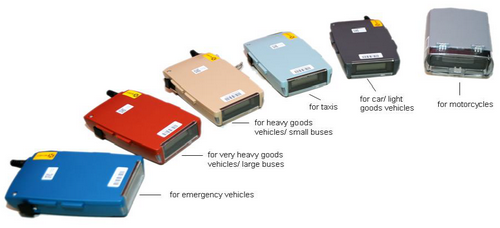
\includegraphics[width=4in]{../img/singapore-IUs.jpg}
	\caption{ERP In-vehicle units \citep{LTA2016}}
	\label{fig:singapore-IUs}
\end{figure}

\begin{figure}
	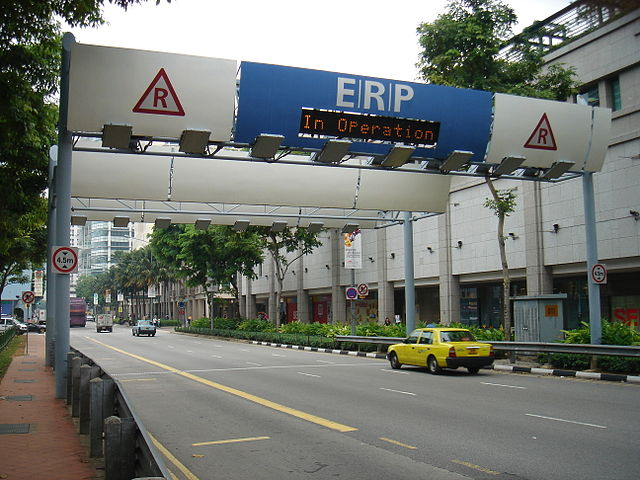
\includegraphics[width=4in]{../img/singapore-gantry.jpeg}
	\caption{ERP gantry \citep{LTA2016}}
	\label{fig:singapore-gantry}
\end{figure}


\begin{figure}
	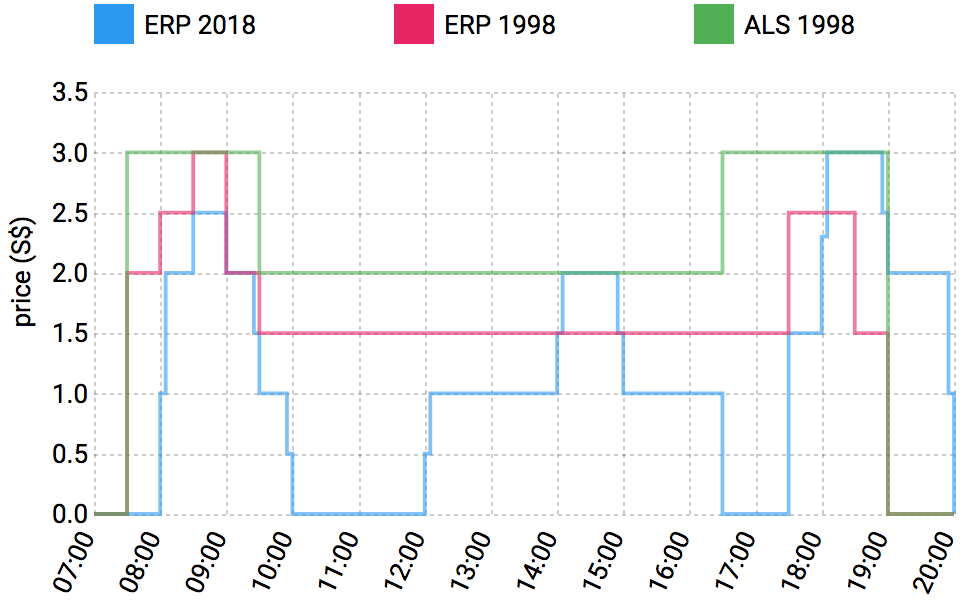
\includegraphics[width=5in]{../img/singapore-prices.png}
	\caption{Singapore prices for different years. The schedule becomes more variable as years pass. }
	\label{fig:singapore-toll-schedule}
\end{figure}

The substantial changes to the design of ERP have been spatial. ERP started in 1998 with 33 gantries that approximately reproduced the ALS cordon. Beginning in 1999, the LTA added gantries gradually to enclose the first cordon in a second ``Outer Cordon'' \citep{Chin2010}. In 2005, a shopping area on the border of the CBD Cordon became a sub-cordon called the Orchard Road Cordon, because shops open later than offices. The same year, gantries were added to charge outbound trips in the evening on one expressway. Finally, in 2008 a line of gantries was planted down the middle of the CBD Cordon. These operate only between 6 and 8PM, when intra-CBD congestion would otherwise be severe. By December 2014, ERP made use of 80 gantries \citep[p. 406]{Chu2015}.

\subsection{Results}

The transition to ERP was not as thoroughly documented as the launch of ALS. One significant effect is that entries to the CBD fell by about 15\%, largely due to a decline in repeat trips by the same vehicle \citep{Menon2000}. Since ALS permitted unlimited same-day entries, under ALS about 23\% of trips had been repeat trips---e.g., office workers using cars for lunches and meetings in the middle of the day \citep[p. 23]{Chin2010}. \citet{Olszewski2005} conclude, using data from before and after ERP, that the LTA's charging structure has done a good job controlling congestion and spreading traffic flow over the peaks.

\subsection{Finances}

ERP is unique among downtown pricing schemes in that its role as a source of revenue is negligible; the entire system is designed for congestion control, as government officials emphasize \citep{Chin2010}. Whereas the Area License Scheme and related Road Pricing Scheme together earned S\$9.3 million per month prior to the switch, ERP earned only S\$5.8 million per month, because ERP tolls were lower than an ALS license \citep[p. 34]{Goh2002}. Singapore does not regularly report revenues, but they were S\$159 million \citep{Chen2012}. ERP revenue is not hypothecated.

Implementation cost S\$197 million in 1998, of which S\$100 million paid for IU's (at a cost of S\$150 each) and S\$97 million to build out the infrastructure (e.g., to buy the gantries) \citep{Santos2004}. Annual operating costs have measured about 20-30 percent of revenues \citep{Chin2010}.
\section{London --- London Congestion Charge}\label{sec:london}

\subsection{Implementation}

Starting with the research described in \citet{Thomson1967a}, the idea of DCP in London became the topic of numerous government studies carried out until the 1990's. These are described in detail in \citet[Ch. 4]{Richards2006} and \citet[Ch. 4]{Gomez-Ibanez1994}. At each study's conclusion, authorities decided to table the matter for the time being, usually citing concerns with technology.

Concrete steps towards a scheme finally began in 1997, when the UK's new Labour government called a referendum on the question of creating a Greater London Authority---a regional governing body over London's many boroughs---to be headed by an elected Mayor of London \citep[Ch. 6]{Richards2006}. In May 1998, this concept won the referendum by a large margin, although it was still up to Parliament to craft specific legislation to create the GLA.\footnote{See \citet[Sec. 7.2]{TfLFifth2007} for a concise list of developments leading up to implementation.} Several Labour policy papers suggested the new Mayor's powers would include enacting road pricing, and so in August 1998 the Government Office for London convened a team of experts, the Road Charging Options for London (ROCOL) Working Group, to study the matter one last time. Around the same time, the UK Treasury decided that it would permit revenues from pricing to be hypothecated to transportation---a break with the usual practice whereby all British government revenues are allocated by the government.  In 1999, Parliament passed the Greater London Authority Act \citep{Parliament1999}, which did give the Mayor road pricing powers, under the proviso that the first ten years of revenue go to transportation. 

In March 2000 ROCOL published its report, \citet{ROCOL2000}, and in May 2000, the first mayoral election went to Ken Livingstone, who had included DCP in his election manifesto (campaign platform). After being briefed on \citet{ROCOL2000}, Livingstone decided to move forward with enforcement by Automatic Number Plate Recognition (ANPR) cameras---a technology perfected in the 1990s. ROCOL had also considered paper licenses and tag-and-beacon systems, but cautioned that the former were impractical and the latter would mean delaying the scheme beyond the Mayor's first term, since national authorities were still working on national standards for transponders. ANPR has the advantage that vehicles do not have to carry special equipment, and has been used in every DCP system except Singapore's.

After preparation and consultation with the public in which several features of the ROCOL plan were modified (e.g., eliminating a proposed higher rate for goods vehicles, granting discounts to residents of the charging zone) the London Congestion Charge went into effect on February 17th, 2003. The launch of the scheme was supported by a permanent expansion of bus service as well as roadwork and traffic signal changes designed to mute the impact of traffic on nearby untolled areas---as described in \cite[p. 132-135]{Richards2006}.

\subsection{Design}

The LCC launched as a \pounds5 charge for unlimited travel between 7:00 AM and 6:30 PM within the 22 km$^{2}$ Congestion Charging Zone (CCZ) (the solid region in Figure \ref{fig:London-Congestion-Charging}). The zone is surrounded by the capacious, uncharged Inner Ring Road which allows drivers to avoid the zone. Uniquely, the LCC covers all travel within the zone---not just traversals of a cordon like the other schemes---as well as vehicles that are merely parked on the street. Therefore, enforcement requires ANPR cameras (over 500 at the launch) mounted on poles throughout the zone and along its boundaries, as well as cameras mounted on patrolling vans. The baseline payment method is as follows: if one uses public streets in the CCZ during charging hours, one has until midnight to pay by calling a number, SMS, a website, payment machines or in various stores. The LCC is turned off from December 25th to January 1st of every years, for Christmas and New Years.


The LCC has undergone a number of minor changes of which we will list only a few. The toll was raised from \pounds5 to \pounds8 in July 2005, \pounds10 in January 2011 and \pounds11.50 in June 2014. In 2007, the end of charging was moved up from 6:30 to 6:00 PM. Since June 2006, if one pays by midnight on the day after visiting the zone the penalty is small (\pounds 2.50). Since 2011, an Auto Pay option lets users have their accounts debited automatically.

The largest, albeit temporary, change to the LCC has been the ``Western Extension,'' a 19 km$^2$ addition to the original CCZ which is shown as the striped area in Figure \ref{fig:London-Congestion-Charging}. After Livingstone was reelected in May 2004, he carried out a consultation with the public on the Extension \citep[Ch. 14]{Richards2006}. The result was soundly negative, but Livingstone chose to proceed anyway, and the Extension came into operation on February 19, 2007. When Boris Johnson defeated Livingstone in the 2008 mayoral election, he conducted another public consultation, \citet{TfL2008b}, on the  Extension. Results showed the public still very opposed, and so the Extension was scrapped on January 4, 2011.

There are myriad exemptions and discounts.\footnote{See \citet[Table 1, p. 515]{Santos2005} for a tabulated list that is almost unchanged today.} Using Auto Pay earns a \pounds1 discount. Residents receive a 90\% discount. Motorcycles, buses, vehicles with 9+ seats, licensed taxis/minicabs, certain emergency and government vehicles, certain vehicles used for or by  disabled people, and certain vehicles with very low emissions are all completely exempt or eligible for a ``100\% discount,'' which, unlike exemption, requires registration and possibly a small fee. The difference between a taxi and minicab is that taxis (also called ``black cabs'') are special black-colored cars that can be hailed from the street, whereas minicabs (also called ``private hire vehicles'') are ordinary cars that can only execute pre-booked pickups. Below, minicabs and private cars are grouped together in statistics---even though the former are exempt---because they are visually indistinguishible from private cars.

\begin{figure}[ht]
    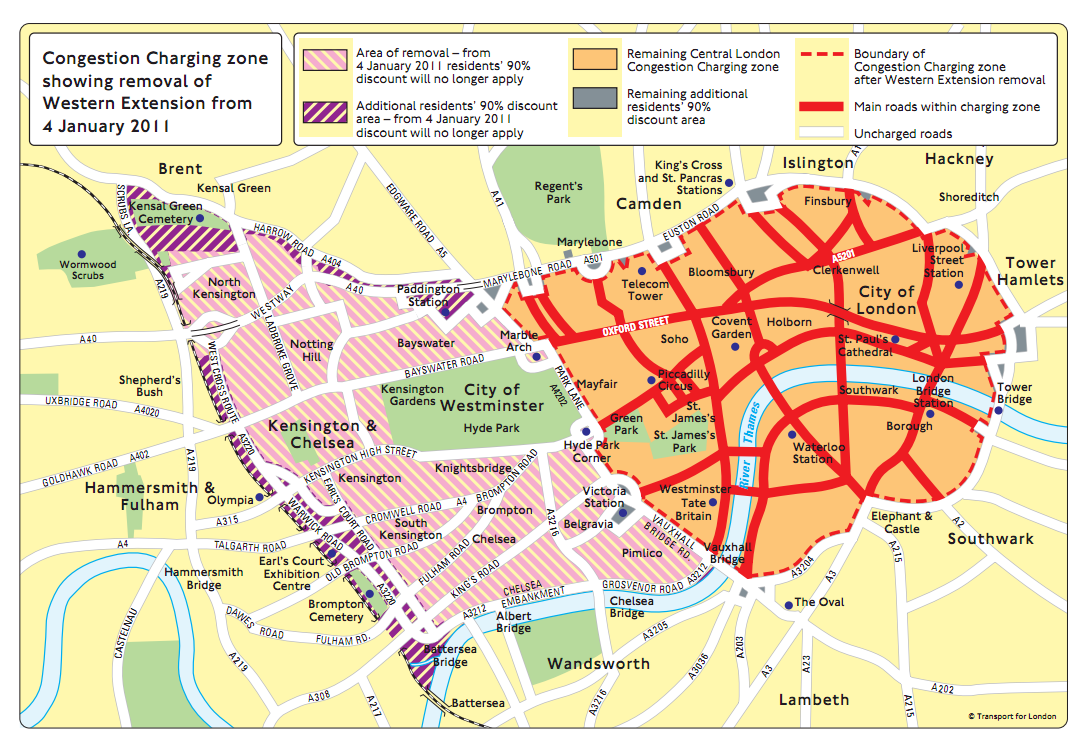
\includegraphics[width=1\textwidth]{../img/london-congestion-charge.png}
    
    \caption{London Congestion Charging Zone \label{fig:London-Congestion-Charging}}
\end{figure}


\subsection{Results}

The LCC is the most closely studied DCP system. Transport for London (TfL) collected data on traffic, travel times, business, transit use and other impacts of the Congestion Charge under the Impacts Monitoring Programme, described in \citet[Sec. 1]{TfLFirst2003}. Findings appear in annual reports from 2003 to 2008, after which more limited data can be found in the TfL's annual Travel in London Report.

The most significant accomplishment of the LCC has beeen to reduce entries to the CCZ and to recompose traffic. See  \ref{fig:london-entries} for entries to the CCZ between 2002 and the first five years of charging. From 2002 to 2003 (before and after the charge), entries by cars and minicabs fell by 33\% (65k) and entries by all potentially-chargeable vehicles (cars/minicabs, trucks and vans) fell 27\% (73k) \citep[p. 22, Tab. 2.2]{TfLFifth2007}. The effect on chargeable traffic was offset by an 18\% (10k) surge in taxi traffic, for a net 18\% fall in entries by all vehicles with 4+ wheels. These patterns held steady through 2007 \citet[p. 41, Tab. 3.1]{TfLSixth2008}. \citet{TfL2017} reports that recent years have seen a steep rise in exempt private hire vehicles, caused by Uber. In response, news reports suggest that London's current Mayor, Sadiq Kahn, is considering removing the minicabs' exemption.
% \footnote{https://www.thetimes.co.uk/article/london-congestion-charge-on-minicabs-to-boost-buses-5kkbqprg9}

% Illustrating Theme II, \citet{TfLDemand2008} note that 


Illustrating Theme II, \citet[p. 19]{TfLFifth2007} remarks, ``Of particular note is the relatively indistinct response to the increase to the daily charge [from \pounds 5 to \pounds 8] in July 2005.'' The next year, TfL published a report on price elasticity noting that the elasticity of demand implied by the toll increase was only -0.16, whereas that implied by the original \pounds 5 toll was -0.51 \citep{TfLDemand2008}.

Results for speed have been more disappointing. (Note first that TfL reports speed changes in terms of the inverse measure min/km, which traffic engineers sometimes call ``pace.'') Before charging, the average pace in the CCZ during charging hours was 4.1 min/km (14.6 kph); in 2003 and 2004 pace fell to about 3.4 min/km (17.6 kph) \citep[Sec. 3.4]{TfLFifth2007}. TfL assumes a baseline, uncongested pace of 1.8 min/km, and so the delay attributed to congestion fell by 30\%. As soon as 2007, however, pace had reverted to its pre-charging level \citep[Sec. 4.4]{TfLSixth2008}. The traffic data firm INRIX reports that, from 2012 to 2015 (inclusive), pace in the CCZ rose by 22\% (i.e., speed fell by 19\%) \citep{INRIX2016}.

TfL has blames falling speed to road work and to capacity-reducing projects such as bus lanes, bus priority and pedestrian or cycling safety measures. The evidence is that similar falls in speed---adjusted for flows---have happened outside the CCZ and at night \citep[Sec. 3.11]{TfLFifth2007}. \citet[p.3]{TfLExPost2007} raises an interesting possibility: ``It is probable that some of these [capacity reallocation] measures have been enabled by charging and would not have happened had charging not reduced traffic levels in the centre of London.'' In this case, the LCC can be looked at not as a way to \emph{raise} traffic speeds but rather as a way to \emph{maintain} traffic speeds while obtaining other public goods and more construction. 

By comparing trends in London against other British cities, \citet{Green2016} find the LCC reduced the number of car accidents per month by 35\%, with the fall explained by both less traffic flow and 22\% fewer accidents per million km-traveled. Areas surrounding the zone exhibited declines as well.

The LCC seems to have boosted bus ridership, although in the long run it is hard to say by how much given that London's bus system has been substantially improved.  From 2002 to 2003, 38\% more bus riders entered the CCZ during the morning; \citet[pp. 40-41]{TfL2004a} attributes half that change to charging and half the bus improvements. \citet[p. 55]{TfL2004a} estimates that, of the 65k car trips diverted between 2002 and 2003, about half switched to bus. In the first year of charging, there was no increase in metro ridership. 

\begin{figure}[ht]
    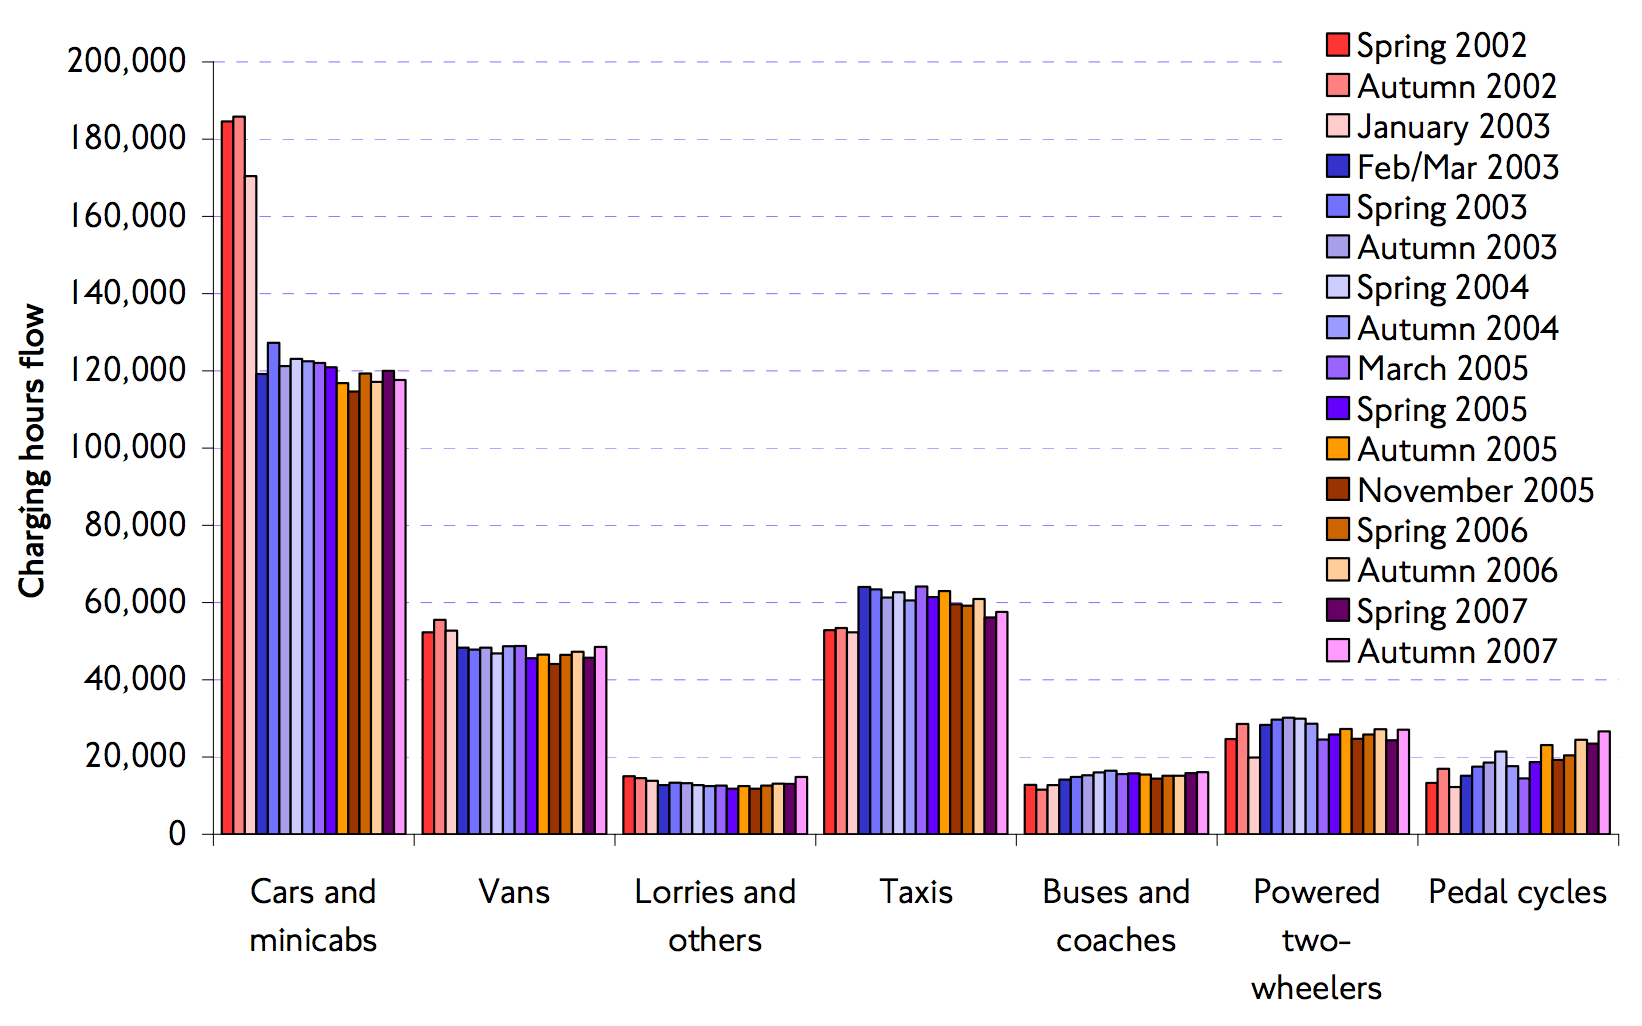
\includegraphics[width=.95\textwidth]{../img/london-entries.png}
    \caption{Entries to the original LCC charging zone by traffic type. \citep[p. 20]{TfLFifth2007} } \label{fig:london-entries}
\end{figure}

\subsection{Finances}
Financially, the LCC has cost more to build and operate and generated, until recently, less money than expected.

\citet[p. 125]{ROCOL2000} predicted setup costs of \pounds30-50 million. In reality, TfL reported implementation costs of \pounds162 million \citep[p. 135]{TfLFifth2007}, but this number requires some context: about \pounds 100 million paid for traffic management measures, including projects for cyclists and pedestrians, bus priority, better signal timing and road improvements \citep[pp. 132-133,138]{Richards2006}. While the LCC may have been the impetus behind these projects, arguably they produced auxiliary own benefits or were to some degree optional. At the same time, this amount does not include the costs of additional public transit provision that went along with the scheme.

As for the yearly budget, \citet{ROCOL2000} estimated annual revenues of \pounds 260-320 million (\pounds 230-270 million from charges and \pounds 30-40 million from penalties) and operating costs of \pounds 30-50 million. ROCOL's plan, however, did not include exemptions for residents or taxis/private hire vehicles; and it imposed a higher charge on delivery vans and trucks. Taking the changes and more realistic costs into account, \citet{TfL2002} projected net revenues of \pounds 130-150 million, not counting penalties.

In reality, operating costs were much higher and revenues lower, as shown in Table \ref{tab:London-Congestion-Charge}. Years 2008-2011 in Table \ref{tab:London-Congestion-Charge} are starred to highlight the years of the Western Extension---a time of higher costs and revenues. \citet[p. 186]{TfL2003b} attributed the shortfall in revenue, initially, to evasion, a greater-than-expected fall in chargeable traffic and the large share of exempt traffic. In 2007, TfL noted that only 44\% of entering vehicles with 4+ wheels were subject to full charge \citep[p. 12]{TfLExPost2007}. Almost as many, 38\%, were made by exempt taxis and private hire vehicles or discounted residents. 

\begin{table}[ht]
    \begin{tabular}{|c|c|c|c|c|c|}
        \hline 
        year & tolls & penalties & revenue & cost & net revenue\tabularnewline
        \hline 
        \hline 
        2003 & 18 & 1 & 19 & 17 & 2\tabularnewline
        \hline 
        2004 & 116 & 55 & 171 & 93 & 78\tabularnewline
        \hline 
        2005 & 117 & 75 & 192 & 90 & 102\tabularnewline
        \hline 
        2006 & 144 & 66 & 210 & 88 & 122\tabularnewline
        \hline 
        2007 & 158 & 55 & 213 & 90 & 123\tabularnewline
        \hline 
        2008{*} & - & - & 328 & 191 & 137\tabularnewline
        \hline 
        2009{*} & - & - & 326 & 177 & 149\tabularnewline
        \hline 
        2010{*} & - & - & 313 & 155 & 158\tabularnewline
        \hline 
        2011{*} & - & - & 287 & 113 & 174\tabularnewline
        \hline 
        2012 & - & - & 227 & 90 & 137\tabularnewline
        \hline 
        2013 & - & - & 220 & 88 & 132\tabularnewline
        \hline 
        2014 & - & - & 235 & 85 & 149\tabularnewline
        \hline 
        2015 & - & - & 257 & 85 & 172\tabularnewline
        \hline 
    \end{tabular}
    
    \caption{London Congestion Charge costs and revenues. Years 2008-2011 are starred to show when the Wesern Extension was in place. 2003-2008 data from TfL's \emph{Congestion Charging Monitoring} reports. Later data from TfL's \emph{Travel in London} series. }\label{tab:London-Congestion-Charge}
\end{table}
\section{Stockholm --- Stockholm Congestion Tax}\label{sec:stockholm}

\subsection{Implementation}

Discussion of downtown pricing in Stockholm started in the 1980s, with a proposal that cars have to display a transit pass in their windshields \citep{GullbergIsaksson2009,Arnott2005}. In 1989, the City of Stockholm formulated plans for this ``car card'' proposal as well as an electronic cordon pricing system \citep[p. 90]{Hau1992}; but since road pricing was deemed a ``tax'' rather than a ``charge,'' Swedish law required that the national parliament approve it. Despite Stockholm's support, parliament tabled the tax for complex political reasons \citep{Ahlstrand2001}. 

Meanwhile, the national government convened Stockholm's political parties to negotiate an infrastructure package. The resulting agreement, finalized in 1992 and called the ``Dennis Package,'' resembled the Norwegian toll ring model: tolls in a cordon around central Stockholm would pay for massive highway and tunnel projects intended to deflect traffic  (see \citet[pp. 39-40]{Gomez-Ibanez1994} and \citet[p. 92]{Hau1992}). However, in 1997 the government cancelled the Dennis Package due, as before, to political maneuvers \citep{Ahlstrand2001,GullbergIsaksson2009}.

In 2000, parliament set up a ``Stockholm Commission'' to  prioritize infrastructure projects, and directed it to reconsider road pricing as source of funds \citep{Eliasson2009b}. As it happened, 2002 was also an election year, and the Moderate Party (Sweden's mainstream conservative party) pounced on the renewed discussion of pricing to win some voters from their rivals, the Social Democrats. In response, a Social Democrat leader, Annika Billstr\"om, announced on television, ``My message to the voters of Stockholm is that there will be no road charging during our next term of office'' \citep{GullbergIsaksson2009}.

The September 2002 election wound up with the Social Democrats and their allies, the Left Party, just short of a majority both nationally and in Stockholm. Seizing the opportunity, the small Green Party made a pact to join the Social Democrat's coallition in exchange for a trial of pricing in Stockholm. The deal sparked a public outcry over Annika Billstr\"om's (by then Mayor of Stockholm) broken pledge, and opponents demanded that the decision of whether to instate pricing permanently be made via referendum. The Social Democrats agreed a referendum would follow the trial's conclusion and appear on the September 2006 election ballot. Originally, the trial was meant to last several years, but political and legal complications delayed the start until January 3, 2006. The trial lasted until July 31, 2006. It was accompanied by a mild transit expansion---mainly of additional bus services--that lasted from September 2005 to December 2007 \citep{Kottenhoff2009}.

Prior to the trial, media coverage of the trial was very negative, and polls showed strong opposition. But once the trial began, public opinion shifted quickly in favor due to very visible congestion reductions.\footnote{A small literature now exists on the question of why public opinion shifted---e.g., XXX LIST SOURCES} At the September 2006 elections, 53\% of Stockholm residents voted to make the scheme permanent. However, at the same election, the leftist coalition lost control of the government at all levels to a center-right alliance of parties who opposed pricing---thus throwing the SCT's future into doubt.  But in the end the new government agreed to respect the referendum results after negotiating a \euro 10 billion infrastructure package, whereby toll revenues were matched by national funds to build new roads---as in the Dennis Package. The SCT returned on a permanent basis on August 1, 2007. In January 2016, tolls were increased and geographically extended.

\subsection{Design}

The Stockholm Congestion Tax (SCT) is a time-variable toll on weekday trips in both directions across a cordon around central Stockholm. See Fig. \ref{fig:stockholm-map} for a map of the tolling sites, which are mostly unchanged. The map has labeled a highway called the Essingeleden; this was originally toll-free for political reasons---being the only north-south route around the city---but in January 2016 it became tolled, although at slightly different rates than in the cordon. The SCT is turned off in July, as Swedes have July off work and traffic is light.

During the trial, the SCT used a radio-frequency tag-and-beacon system backed up by ANPR cameras, but with time the error rate for ANPR became low enough that transponder enforcement was ended in late 2008 \citep[p. 841]{Hamilton2011}. Vehicles are charged when they cross under metal gantries, which work as a trio: when a laser on the middle gantry detects a vehicle, cameras mounted on the first and third photograph the front and rear plates.\footnote{``Frequently asked questions about congestion tax.'' \emph{https://transportstyrelsen.se/en/road/Congestion-taxes-in-Stockholm-and-Goteborg/frequently-asked-questions-about-congestion-tax/}}

Figure \ref{fig:stockholm-prices} displays the current charging schedule, alongside that of Gothenburg's. Originally, tolls during the peaks were about 2/3 of their current values, but in 2016 the charge was increased to fund an infrastructure package \citep{Borjesson2018}. Although vehicles are ostensibly charged for each cordon passage, there is a maximum daily charge, beyond which traversals are free; the maximum was 60 SEK until the 2016 toll increase but is now 100 SEK. 

Today, emergency vehicles, diplomatic vehicles, vehicles for disabled person and and buses weighing at least 14 metric tonnes are exempt. Vehicles registered abroad were exempt until 2015.\footnote{http://urbanaccessregulations.eu/news-and-press/swedish-congestion-charge-now-applies-to-foreign-vehicles } Alternative-fuel vehicles were exempt until 2012. Taxis were exempt only during the trial. Trips going directly between the island of Liding\"o (the starred island in Fig. \ref{fig:stockholm-map}) are exempt, since Liding\"o can only be accessed via the SCT zone. Such direct trips are identified as trips that cross two tolling sites within thirty minutes, with one of the two being among the tolling sites at the Liding\"o. Until recently, companies were allowed to pay the toll for employees driving company cars (about one quarter of cordon crossings) as an untaxed fringe benefit, which, given Sweden's high taxes, significantly diminished the toll; but as of 2018 new legislation has ended this practice \citep[Sec. 2.2]{Borjesson2018}.

\begin{figure}
    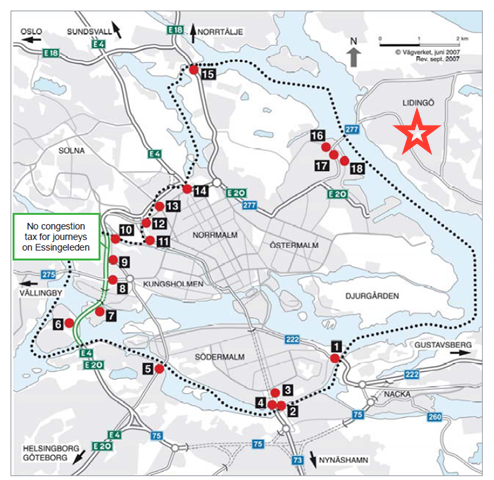
\includegraphics[width=5in]{../img/stockholm-map.png}
    \caption{Stockholm Congestion Tax, access points in red. \citep{transportstyrelsen2015}}
    \label{fig:stockholm-map}
\end{figure}

\begin{figure}
    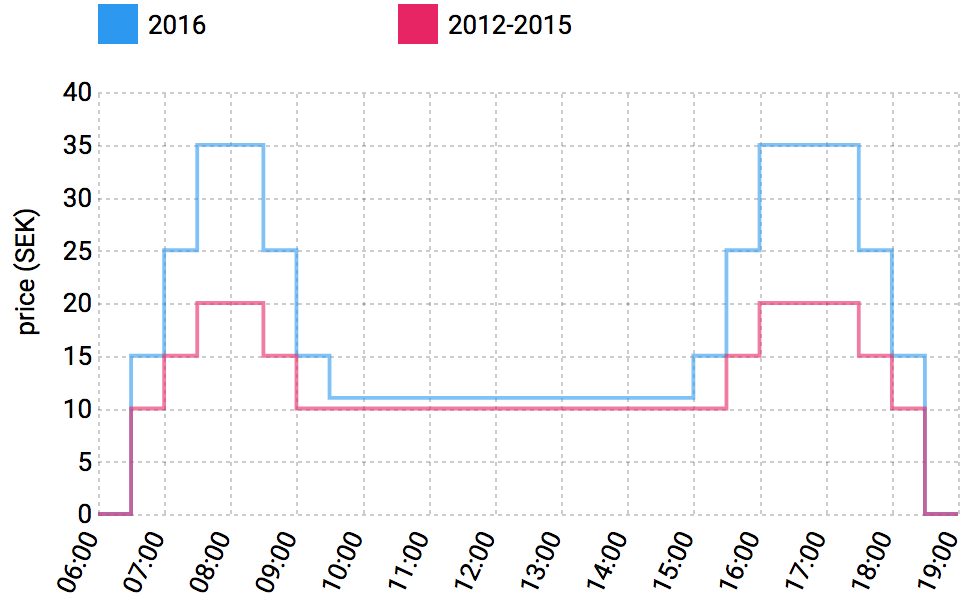
\includegraphics[width=4.5in]{../img/stockholm-prices.png}
    \caption{Stockholm toll schedule }
    \label{fig:stockholm-prices}
\end{figure}

\subsection{Results}

During the trial, flows across the cordon during charging hours fell by about 20\% in both the peaks and the mid-day off-peak, exceeding the 16\% drop that had been forecast \citep{Eliasson2013}. After the reintroduction of the charge, and despite growth in Stockholm, cordon flows remained almost constant \citep[Tab. 4]{Borjesson2018}. The share of exempt traffic hovered between 25\% and 28\% from 2008 to 2011, but thereafter declined to about 15\% due to the removal of the exemption for electric vehicles. 

Theme II appears again in that, after the 2016 price increase, cordon traversal  during the peaks fell only 5\%, despite charges almost doubling \citep[p. 43, Tab. 6]{Borjesson2018}. The authors calculate the price elasticity of demand from the charge increase to be only 30\% of the elasticity implied by the introduction of charging.

During the trial, taxis---which were exempt---were expected to account for 4\% of traffic, but actually acounted for 8\% \citep{Eliasson2013}. This result accords with the early experience in Singapore and London, where taxi entries surged.

Using survey data for the trial, \citet{Franklin2008} find the fall in person-trips was similar for commuters (24\%) and discretionary travelers (22\%), but the two groups adapted differently: commuters who stopped driving switched to public transit, while discretionary travelers cancelled or rerouted their trips. 

Travel time savings exceeded forecasts substantially, mainly due to reductions in queues which traffic forecasters had trouble modelling \citep{Eliasson2013}. Figure \ref{fig:stockholm-travel-time} shows delays recorded on different roads; as the figure shows these gains gains persisted over the years they were measured.

\begin{figure}
    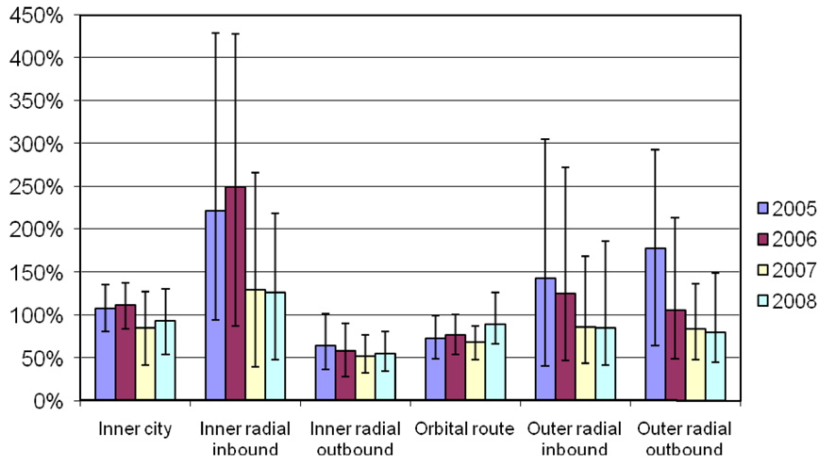
\includegraphics[width=\textwidth]{../img/stockholm-travel-times.png}
    \caption{Sweden price structure \citep{Borjesson2012} XXX INCLUDE NOTE LATER EXPLAINING THE METRIC. Note that the orbital route lies outside the cordon.}
    \label{fig:stockholm-travel-time}
\end{figure}

\citet{Simeonova2017} finds robust evidence that the Congestion Tax caused a 5-10 percent decline in air pollution, which led to a 47\% fall in the rate of urgent care visits for children with asthma.



\subsection{Finances}

The cost of the charging system trial was 1900 MSEK, of which 1050 MSEK was spent prior to the start of charging \citep{Eliasson2009}. Another 1400 MSEK paid for the public transit expansion---mostly to buy 200 buses and run extra bus lines until December 2007 \citep[p. 398]{Eliasson2008}.

\citet{Hamilton2011} describes several factors that explains the high cost of implementation. First, transaction costs were originally high because every charge was processed separately. Second, the Liding\"o exemption required an expensively low false negative rate (achieved by manually double-checking video), because if the system identifies a Liding\"o trip when it enters the cordon but misses it leaving (or vice versa), then it charges the exempt trip.\footnote{Jones Eliason, a researcher involved in the implementation, has remarked, ``Had we realized just how expensive the Liding\"o exception would be, it is unlikely that it would have been adopted'' \citep[p. 217]{Eliasson2009b}.} Third, delay caused by legal and political complications wasetd contractors' time. Finally, having such a short trial required expensive redundancy and overdesign, because the system had to work perfectly and immediately with little testing.


 SCT has since become very profitable. In 2008, operating costs were 220 MSEK and revenues 710 MSEK, but by 2016 operating costs were down to 103 MSEK and revenues up to 1400 MSEK \citep[p. 40]{Borjesson2018}. Revenues during the trial were 14\% less than expected, which \citet{Eliasson2013} explain is partly due to underestimating the fall in demand but mainly due to a higher-than-expected share of exempt traffic.


\section{Milan --- Area C}

\subsection{History}

The Milan experience with downtown pricing depends on two pieces of context. First, Italian cities commonly operate ``limited traffic zones'' (ZTL's), areas where vehicle access is restricted. A ZTL, for instance, might ban private vehicles during the workday except for residents. Milan already had a camera-enforced ZTL inside its Cherchia dei Bastioni, a ring of 16th century fortifications around the city center, so charging required less new infrastructure and planning. Second, Milan has relatively high use of cars and motorcycles and sits in the relatively windless Po Valley, leading to severe particulate pollution \citet{Rotaris2010}.

During his 2002-2007 term, Milan's Mayor, Gabriele Albertini, discussed charging for access to the Cerchia dei Bastioni, and his replacement, Letizia Moratti, took up the cause following her election in 2006 \citep{Mattioli2012}. These plans bore fruit with the January 1, 2008 launch of ``Ecopass,'' an camera-enforced daily license scheme aimed at curbing high-emission vehicles. Ecopass had a complex charging structure (see Table \ref{tab:milan-ecopass-prices}) and liberal exemptions that made entry free for many vehicles. Thus, the share of chargeable vehicles entering the zone fell from 42 percent before Ecopass to just 16 percent by 2009 \citep[p. 5, Table 3]{Danielis2011}. Observers believed Ecopass was not having its advertised effect, particularly since air pollution worsed in early 2010 \citep{Mattioli2012}. Consequently, in 2010 activists helped to organize a petition drive for a number of environmental and transportation referenda, including a strengthening of Ecopass. In July 2011, all the referenda passed, with 79 percent for the Ecopass proposal. Around the same time, Moratti was replaced as mayor by Giuliano Pisapia, who set about remaking Ecopass. The reorganized system, called Area C, has operated since January 1, 2012 with a simpler structure (See Table \ref{tab:milan-area-c-prices}) oriented more toward congestion reduction. 

\subsection{Design}

The charging zone of both Area C is an 8 km$^{2}$ area of central Milan called the Cerchia dei Bastioni (see Figure \ref{fig:milan-map}). The cordon consists of 43 access points where cameras read the number plates of entering vehicles. Charging operates from 7:30 AM and 7:30 PM on weekdays \citep{Milan2015}. The standard way to pay is to buy a digital ``ticket'' at banks, parking meters, online, ATM's or in stores and then ``activate it''---that is, associate it with a plate number on a particular day---by phone, SMS, online or at municipal offices. Since the switch to Area C, users can also sign up for a Telepass radio-frequency transponder to pay by debit automatically. What most distinguishes Ecopass from Area C is the charging structure: Ecopass involved a schedule of emission classes , while Area C involves a schedule of user classes. See Tables \ref{tab:milan-ecopass-prices} and \ref{tab:milan-area-c-prices} below. Both systems have also come with an enormous number of exemptions, including motorcycles and scooters, a certain number of free days for residents and vehicles delivering  perishable and refrigerated food \citet{Danielis2011}. Ecopass also offered residents of the zone a 50\% discount on their first 50 entries per year, and a 40\% discount on the next fifty.

\begin{figure}[ht]
	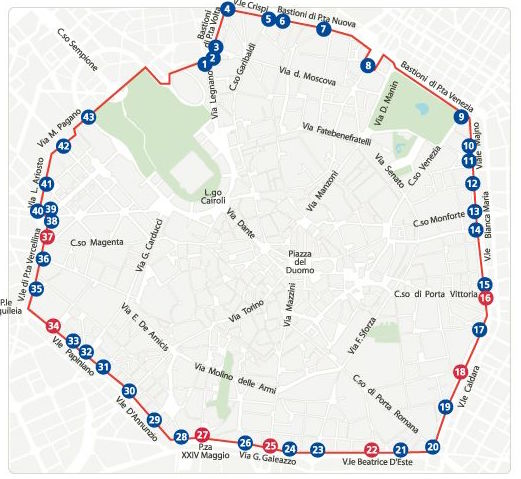
\includegraphics[width=.64\textwidth]{../img/milan-map.jpg}
	\caption{Milan Ecopass/Area C \citep{Rotaris2010}}
	\label{fig:milan-map}
\end{figure}

\begin{table}
\begin{center}
\begin{tabular}{|>{\centering}m{1.8cm}|>{\centering}m{1.8cm}|>{\centering}p{1.8cm}|}
\hline 
Emissions Class & Charge (\euro) \tabularnewline
\hline 
\hline 
1 & 0 \tabularnewline
\hline 
2 & 0 \tabularnewline
\hline 
3 & 2 \tabularnewline
\hline 
4 & 5 \tabularnewline
\hline 
5 & 10 \tabularnewline
\hline 
\end{tabular}
\par\end{center}
\caption{Ecopass prices. Lower classes are less polluting. Class I includes hybrid and electric cars. Class V low-efficiency diesel and buses. \citep{Rotaris2010} }\label{tab:milan-ecopass-prices}
\end{table}

\begin{table}

\begin{center}
\begin{tabular}{|>{\centering}m{2.2cm}|>{\centering}m{1.8cm}|}
\hline 
User Class & Charge (\euro)\tabularnewline
\hline 
\hline 
standard & 5\tabularnewline
\hline 
residents & 2\tabularnewline
\hline 
commercial & 3\tabularnewline
\hline 
\end{tabular}
\par\end{center}
\caption{Area C prices \citep{Milan2015}}\label{tab:milan-area-c-prices}
\end{table}

\subsection{Results}

During the Ecopass trial, congestion inside the cordon fell by 12.3\%, vehicle-kilometers traveled by 14.2\% and accidents by 20.6\% while bus speeds and private vehicle speeds rose, respectively, 7.8\% and 4\% \citep{Rotaris2010}. Using time-series data during the suspension in summer 2012, \citet{Gibson2015} estimate that the suspension raised entries to the charging zone during charging hours by 27,500 per day (14.5 percent), CO concentrations by 6 percent and PM10 concentrations by 17 percent.

\section{Gothenburg --- Gothenburg Congestion Tax}\label{sec:gothenburg}

\subsection{Implementation}

The genesis of Gothenburg's pricing system lies in the above-mentioned infrastructure agreement between Stockholm and the national government. Previously, most infrastructure projects in Sweden were funded nationally, but the agreement demonstrated a local/national co-financing model \citep{Borjesson2015,Hysing2015b}. In 2008 the government directed the infrastructure administration to prioritize such co-financing when selecting projects for the 2010-2021 transport investment plan. When a draft of the plan came out in spring 2009, leaders from the Gothenburg region lamented that many of their high-priority projects had been left out, and embarked on negotiations with national officials about co-financing these projects. The negotiations proceeded quickly, and in October 2009 the Gothenburg City Council ratified the ``West Swedish Agreement,'' whereby 17 billion SEK in local funds---including 14 billion from road pricing---would be matched one-for-one by national funds.\footnote{http://www.vastsvenskapaketet.se/english/} The Agreement included a 20 billion SEK rail tunnel (the ``Western Link''), a road tunnel, bus lanes and a multi-modal bridge. 

Unlike the protracted process behind the Stockholm Congestion tax, the selection of projects and the design of the road pricing scheme were both rushed, so that the projects could be included in the national investment plan that Parliament passed in April 2010. This provoked controversy, and in the September 2010 elections, voters gave several seats on the Gothenburg City Council to a new party, Vägvalet (``Road Selection''), whose sole issue was opposition to road pricing. In 2012, a public petition drive led the council to  place a on-binding referendum on the coming charges on the 2014 election ballot. Nevertheless, the Council pressed ahead, and the Gothenburg Congestion Tax (GCT) launched on January 1st, 2013 with a design copied from the SCT. In September 2014, the referendum result showed 57\% of votes cast were against continuing the charge, but since the referendum was only consultative, the Council decided to keep the Tax in order to fulfill Gothenburg's end of the West Swedish Agreement. This motive has been well illustrated by the decision to increase tolls in January 2015 after early revenues fell short of projections.

\subsection{Design}

Gothenburg's scheme uses the same technology and design as Stockholm's: cameras identify drivers crossing tolling sites in either direction, and tolls vary by time-of-day. Figure \ref{fig:gothenburg-prices} shows the tolling schedule in place today, which is somewhat larger than the original schedule. There is a daily maximum charge of 60 SEK, and the same vehicles are exempt as in Stockholm. Figure \ref{fig:Gothenburg-map} shows the tolling sites form a cordon around downtown Gothenburg, but there are also sites at the \"Alvsborg Bridge (toll site \#11) and along a highway north of the city where congestion would otherwise be severe. Note that more tolling sites are required for Gothenburg than for Stockholm owing to the lack of water boundaries.

Gothenburg has the same exemptions has Stockholm, and the Tax is turned off in July. One feature unique to Gothenburg's scheme is the ``single charge'' or  ``multi-passage'' rule: no matter how many tolling sites a vehicle crosses within 60 minutes, it is charged only once, with the toll being the highest among the possible charges. 

\begin{figure}[ht]
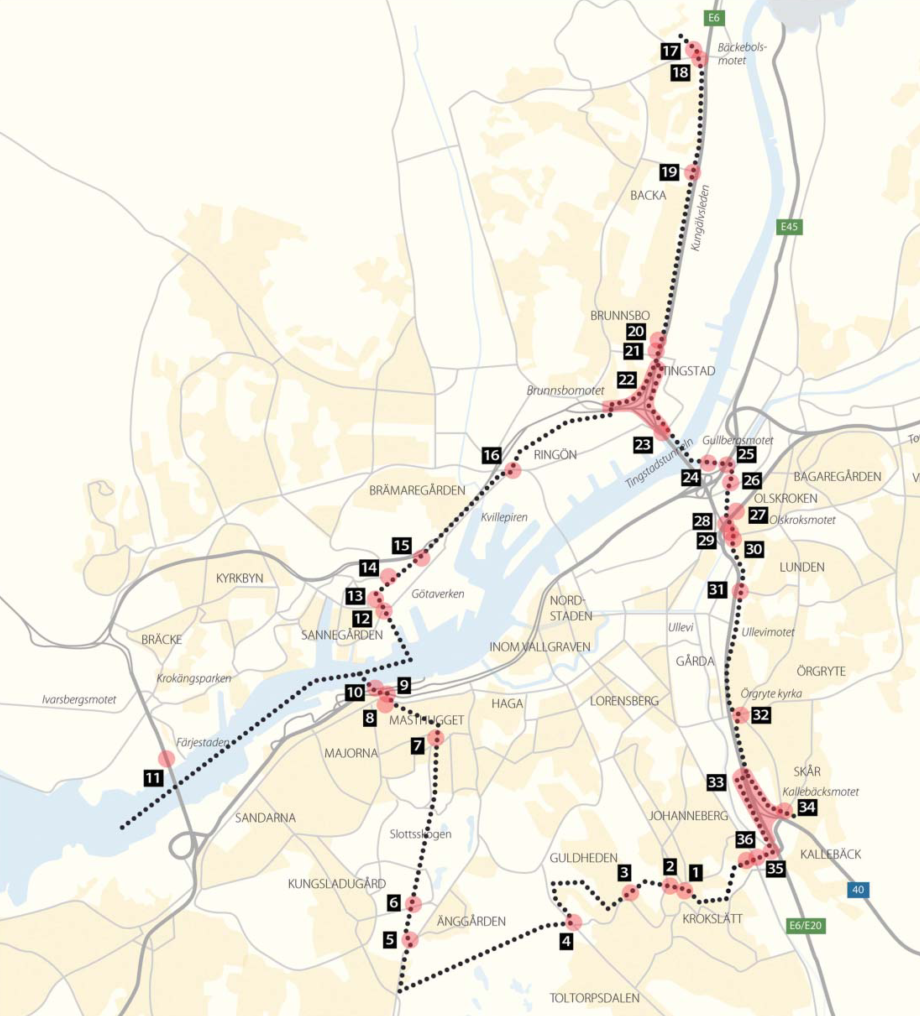
\includegraphics[width=0.7\textwidth]{../img/gburg-map.png}
\caption{Gothenburg Congestion Tax zone \citep{transportstyrelsen2015}\label{fig:Gothenburg-map}}
\end{figure}

\begin{figure}
    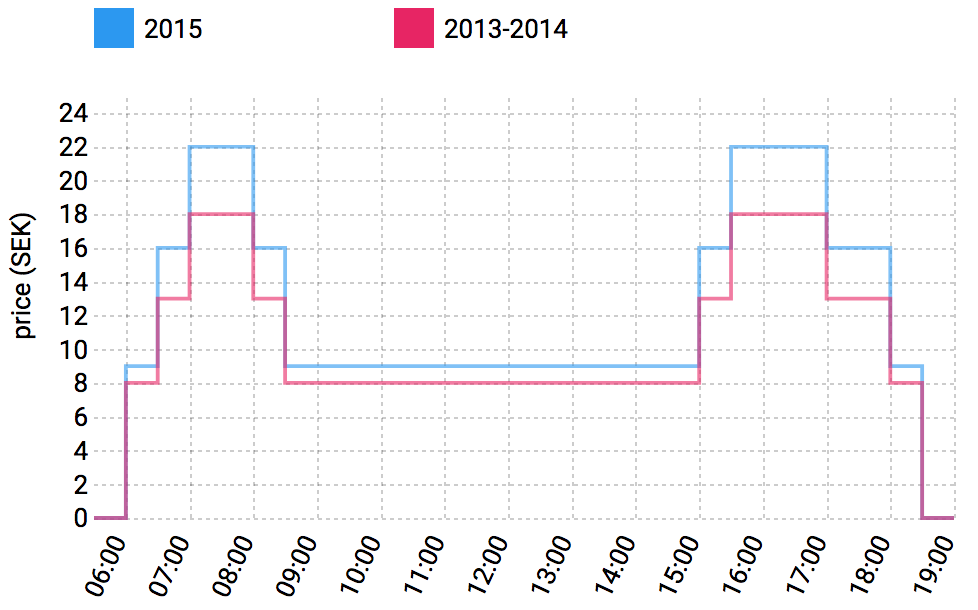
\includegraphics[width=0.8\textwidth]{../img/gothenburg-prices.png}
    \caption{Gothenburg price structure } 
    \label{fig:gothenburg-prices}
\end{figure}

\subsection{Results}

Between 2012 and 2013, cordon crossings during charging hours fell 12\%, rather than the 15\% forecast by models \citep{Borjesson2015}. Although peak crossings were expected to fall more than off-peak, due to the higher charges, in fact both fell by about 12-13\%. (Recall that Stockholm also surprised observers by showing the same reduction in the peak and off-peak.) Entries have been stable since enactment \citet[Tab. 5]{Borjesson2018}.

Travel time savings were mild---mostly because Gothenburg was not very congested in the first place. Results appear in Fig. \ref{fig:Gothenburg-travel-times}. Inner arterials are the highways circled in Fig. \ref{fig:Gothenburg-map}; outer arterials are the uncircled highways outside the zone; bypasses are highways further out than the map shows. As the figure shows, congestion intitially was much lighter than it was in Stockholm, and there very little change in traffic within the cordon. The dramatic reduction on the inner arterials is attenuated by the fact that travel time on these links had only been about 5 minutes during the morning peak. 

Surveys conducted before and after charging show that commuters switched to public transport, while discretionary travelers traveled less frequently or switched destinations. Accounting for external factors, the charge is estimated to have raised public transport ridership by about 4.5-6.5\% \citep{Borjesson2015}.

\begin{figure}[ht]
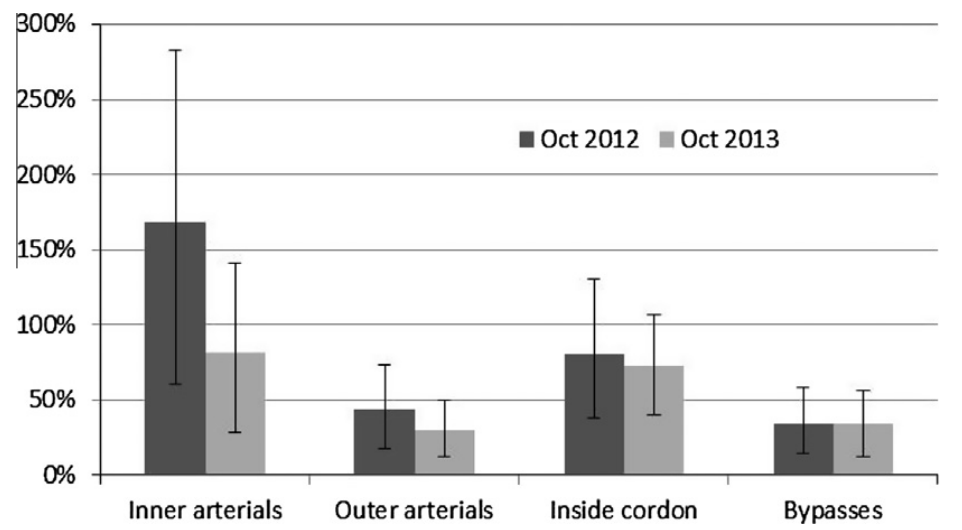
\includegraphics[width=0.55\columnwidth]{../img/gburg-travel-times.png}

\caption{Gothenburg 6-10 A.M. Increase in travel times on selected categories of road relative to free-flow speeds, before (Oct 2012) and after (Oct 2013) the Congestion Tax. \citep{Borjesson2015} \label{fig:Gothenburg-travel-times}}

\end{figure}

Like Stockholm, Gothenburg confirms Theme II: the 2015 toll increase resulted in no real change in entries during the peak hours, although the increase was not as substantial as in Stockholm \citep[p. 43, Tab. 6]{Borjesson2018}.

\subsection{Finances}

The GCT cost only 410 MSEK to implement if we count only those costs specific to Gothenburg \citep[p. 40]{Borjesson2018}. However, in 2012, Sweden spent 350 MSEK to replace the IT system for the Stockholm Congestion Tax with a national system that Gothenburg and two bridges elsewhere in Sweden could also use; arguably some part of this expense could be attributed to Gothenburg. 

In the first year, 2013, the GCT earned 720 MSEK in charges and about 8 MSEK in penalties---13 million short of the amount that had been forecast forecast in 2009 \citep[pp. 142-143]{Borjesson2015}. \citet{Borjesson2015} blame the shortfall on economic factors (fuel prices, recession) and the fact that 45\% of trips into the cordon during charging hours took advantage of the ``multi-passage'' rule---rather than the 30\% analysts predicted. The shortfall is what led authorities to raise the toll in 2015, since---unlike in London where revenues are hypothecated to transit in a vague way---the Western Swedish Agreement commits Gothenburg to pay for specific projects. The increase led revenues to jump from 80 MSEK in 2014 to 99.5 million EUR in 2015. Operating costs have been around 130 MSEK per year and are declining \citep[table 3]{Borjesson2018}.





\section{The future}\label{sec:future}

The story of DCP is certainly unfinished. There are now several important developments underway, including revamping of extant schemes and the possible implementation of new ones.

The most likely source of major developments is Singapore. Singapore has already started the process of changing ERP into ERP 2.0, a distance-based charge, administered by satellite tracking and roadside cameras.\footnote{http://www.straitstimes.com/singapore/transport/erp-20-goes-the-distance-with-new-tech} The new system is planned to launch in 2020, and will also incorporate parking charges.

In London, the LCC infrastructure is being purposed for pollution control. On October 23, 2017, TfL commenced operation of the ``T-charge'' system. This scheme charges an additional \pounds 10 to older vehicles with higher emissions to enter the CZ during the same charging period as the LCC.\footnote{ ``T-Charge: New London traffic charge comes into force'' http://www.bbc.com/news/uk-england-london-41695116} The measure is a step on the way to the April 2019 implementation of an ``Ultra-Low Emission Zone,'' which would enact much higher charges (e.g., up to \pounds 100 for certain trucks) on a broader range of vehicles than the T-Charge (including motorcycles) and apply 24 hours every day of the year.\footnote{``Ultra Low Emission Zone'' https://tfl.gov.uk/modes/driving/ultra-low-emission-zone} London Mayor Sadiq Kahn has also entertained the idea of replacing the LCC with a distance-based charge.\footnote{https://www.citylab.com/transportation/2017/06/london-driving-mileage-fee-sadiq-khan/531270/}

The Swedish Ministry of Finance recently proposed to increase the Stockholm Congestion Tax, by 10 SEK at the peaks (28\%), and to extend charging to more days of the year.\footnote{https://mitti.se/nyheter/trafik/forslaget-dyrare-trangselskatt/?omrade=hela-stockholm} The Stockholm government is receptive to the idea as long as revenues are invented in local transportation.

In Vancouver, local governments and the regional transportation authority (TransLink) have established a special commission tasked with researching options for congestion pricing. Their first report, \citep{vancouver2018}, considers---among more traditional scheme designs---implementing DCP using a distance-based charge. 

In Fall of 2017, Andrew Cuomo, governor of the state of New York, appointed a task force called FixNYC to reexamine at DCP for lower Manhattan.\footnote{https://www.nytimes.com/2018/01/16/nyregion/cuomos-congestion-pricing-for-new-york-city-begins-to-take-shape.html} The task force has yet to release a report, but it reportedly will incorporate a cordon toll as well as distance- and time-based levies on taxis and ridesharing vehicles.


% ERP 2.0

% The San Francisco County Transportation Authority is currently running a long-term study 

% SAN FRANSCISCO MAPS STUDY. NEW YORK CITY. VANCOUVER.

\section{Discussion}\label{sec:discussion}

This chapter has reviewed the history of zone pricing from its conception as an idea in the 1950's and 1960's to its proliferation in the new millenium as a result of number-plate recognition technology. Surveying the zone pricing experience, two themes emerge that are worth highlighting.

First, note that all the systems surveyed produced similar traffic reductions, between 10 and 20 percent of all entries. This is surprising given that the amount of money charged varies considerably. In Stockholm, the maximum charge is only about \$3. In London it was about \$18 before the recent devaluation of the pound. Moreoever, the models in Stockholm and Gothenburg were mistaken in that they predicted different traffic reductions in the peak and off-peak, due to the time-varying toll. Instead what was observed is that a similar share of traffic stopped driving at both times of day. As a rule-of-thumb, it might be worthwhile to assume that, in any pre-charging population of drivers, about 10-15\% of drivers are simply unwilling to pay anything to drive, almost regardless of the size of the toll.

Second, while most of the theory of congestion pricing focuses on prices, in practice exemptions are critical. Some of these exemptions---such as those for the handicapped or medical vehicles---are easy to justify by appeals to welfare or social justice. But many exemptions---such as those for taxis or even, in the case of Milan, refrigerated delivery trucks---lack much of a rationale outside politics.

\pagebreak
\subsection*{References}
\bibliographystyle{apalike}
\bibliography{../../papers/practice}

\end{document}